\documentclass[12pt, notitlepage, final]{article} 

\newcommand{\name}{Vince Coghlan}

\usepackage{amsfonts}
\usepackage{amssymb}
\usepackage{amsmath}
\usepackage{latexsym}
\usepackage{enumerate}
\usepackage{amsthm}
\usepackage{nccmath}
\usepackage{setspace}
\usepackage[pdftex]{graphicx}
\usepackage{epstopdf}
\usepackage[siunitx]{circuitikz}
\usepackage{tikz}
\usepackage{float}
\usepackage{cancel}
\usepackage{pgfplots}
\usepackage{setspace}
\usepackage{overpic}
\usepackage{mathtools}
\usepackage{listings}
\usepackage{color}

\numberwithin{equation}{section}
\DeclareRobustCommand{\beginProtected}[1]{\begin{#1}}
\DeclareRobustCommand{\endProtected}[1]{\end{#1}}
\newcommand{\dbr}[1]{d_{\mbox{#1BR}}}
\newtheorem{lemma}{Lemma}
\newtheorem*{corollary}{Corollary}
\newtheorem{theorem}{Theorem}
\newtheorem{proposition}{Proposition}
\theoremstyle{definition}
\newtheorem{define}{Definition}
\newcommand{\column}[2]{
\left( \begin{array}{ccc}
#1 \\
#2
\end{array} \right)}

\newdimen\digitwidth
\settowidth\digitwidth{0}
\def~{\hspace{\digitwidth}}

\setlength{\parskip}{1pc}
\setlength{\parindent}{0pt}
\setlength{\topmargin}{-3pc}
\setlength{\textheight}{9.0in}
\setlength{\oddsidemargin}{0pc}
\setlength{\evensidemargin}{0pc}
\setlength{\textwidth}{6.5in}
\newcommand{\answer}[1]{\newpage\noindent\framebox{\vbox{{\bf ECEN 4797 Fall 2014}
\hfill {\bf \name} \vspace{-1cm}
\begin{center}{Homework \#4}\end{center} } }\bigskip }

%absolute value code
\DeclarePairedDelimiter\abs{\lvert}{\rvert}%
\DeclarePairedDelimiter\norm{\lVert}{\rVert}
\makeatletter
\let\oldabs\abs
\def\abs{\@ifstar{\oldabs}{\oldabs*}}
%
\let\oldnorm\norm
\def\norm{\@ifstar{\oldnorm}{\oldnorm*}}
\makeatother

\def\dbar{{\mathchar'26\mkern-12mu d}}
\def \Frac{\displaystyle\frac}
\def \Sum{\displaystyle\sum}
\def \Int{\displaystyle\int}
\def \Prod{\displaystyle\prod}
\def \P[x]{\Frac{\partial}{\partial x}}
\def \D[x]{\Frac{d}{dx}}
\newcommand{\PD}[2]{\frac{\partial#1}{\partial#2}}
\newcommand{\PF}[1]{\frac{\partial}{\partial#1}}
\newcommand{\DD}[2]{\frac{d#1}{d#2}}
\newcommand{\DF}[1]{\frac{d}{d#1}}
\newcommand{\fix}[2]{\left(#1\right)_#2}
\newcommand{\ket}[1]{|#1\rangle}
\newcommand{\bra}[1]{\langle#1|}
\newcommand{\braket}[2]{\langle #1 | #2 \rangle}
\newcommand{\bopk}[3]{\langle #1 | #2 | #3 \rangle}
\newcommand{\Choose}[2]{\displaystyle {#1 \choose #2}}
\newcommand{\proj}[1]{\ket{#1}\bra{#1}}
\def\del{\vec{\nabla}}
\newcommand{\avg}[1]{\langle#1\rangle}
\newcommand{\piecewise}[4]{\left\{\beginProtected{array}{rl}#1&:#2\\#3&:#4\endProtected{array}\right.}
\newcommand{\systeme}[2]{\left\{\beginProtected{array}{rl}#1\\#2\endProtected{array}\right.}
\def \KE{K\!E}
\def\Godel{G$\ddot{\mbox{o}}$del}

\onehalfspacing

\begin{document}

\answer{}

\textbf{4.1:}
An IGBT and a silicon diode operate in a buck converter, with the IGBT waveforms in Fig 4.57. The converter
operates with input voltage $V_g = 400V$, output voltage $V=200V$, and load current $I=10A$.
\begin{figure}[H]
\begin{center}
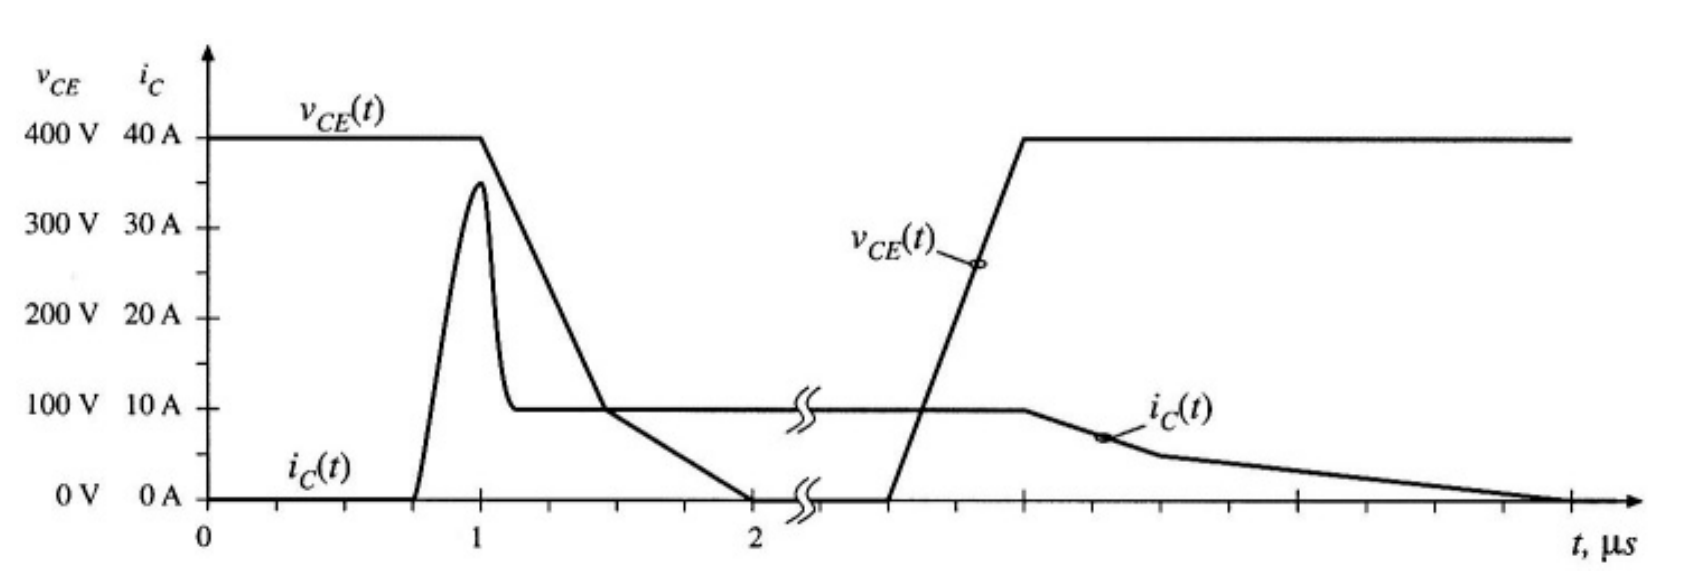
\includegraphics[width=14cm]{f1}
\end{center}
\end{figure}
\begin{enumerate}[(a)]
  \item{Estimate the total energy lost during the switching transitions}\\
    power loss is going to be voltage times current.  Energy will be power times time. I will devide
    the graph into 7 sections, treating the begining of the waveform as a linear line:
    This means that we can easily estimate the total energy for the first section.
    \[
      E = 2.5\cdot10^{-7}\cdot(400\cdot17.5) = 1.75mJ
    \]
    Finding the rest of them shows that:
    \[
      E_{\text{loss}} = 1.75mJ+1.06mJ+0.23mJ+0.25mJ+1mJ+1.5mJ+1.5mJ = 7.29mJ
    \]

  \item{The forward voltage drop of the IGBT is 2.5V, and the diode has forward voltage
    drop 1.5V.  All other sources of conduction loss and fixed loss can be neglected.
    Estimate the semiconductor conduction loss.}\\
    The semiconductor loss will be the power lost when the load current is on (all of the
    diode currents will go through the load).  This looks like (remember only one
    of the devices will conduct at a time):
    \[
      P = I\cdot V = D\cdot 10\cdot 2.5 + D'\cdot 10\cdot 1.5 = 25D + 15D'
    \]
    With this information, we can solve for $D$. If this is an ideal Buck Converter, than the
    ratio of voltage out over voltage in will be equal to the duty cycle.  This means that
    our duty cycle is 0.5, and our power lost is 20W.

  \item{Sketch the converter efficiency over the range of switching frequencies $1\text{kHz}
    \leq f_g \leq 100\text{kHz}$}, and label numerical values.\\
    Efficiency is defined as $\frac{P_{\text{out}}}{P_{\text{in}}}$ and can be calculated as:
    \[
      \eta = \frac{P_{\text{out}}}{P_{\text{out}}-P_{\text{loss}}-P_{\text{switch}-P_{\text{switch}}}}
    \]
    \[
      \eta = \frac{200\cdot10}{200\cdot10 - 20 - 0.00175\cdot f}
    \]
    This looks like:
    \begin{figure}[H]
    \begin{center}
    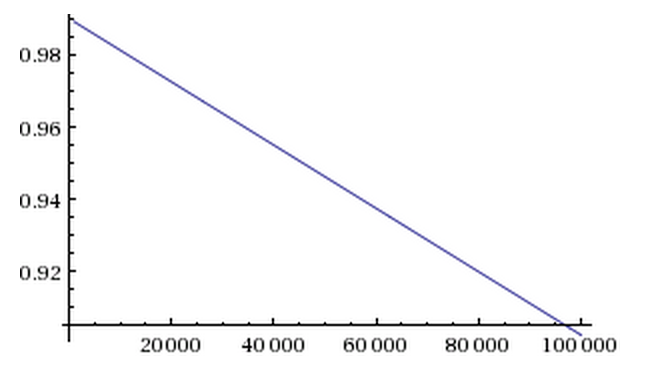
\includegraphics[width=8cm]{f2}
    \end{center}
    \end{figure}

\end{enumerate}


\textbf{4.2:} The buck-boost converter shown below is implemented with a MOSFET and a diode. The
MOSFET can be modeled as ideal, but the diode exhibits “snappy” reverse-recovery
characteristics, with reverse recovery time $t_r$ and recovered charge $Q_r$.
In addition, the inductor has winding resistance $R_L$. The converter operates
with small inductor current ripple and small capacitor voltage ripple.
Derive an equivalent circuit that models the dc components of the converter waveforms and
that accounts for the loss elements described above.
\begin{figure}[H]
\begin{center}
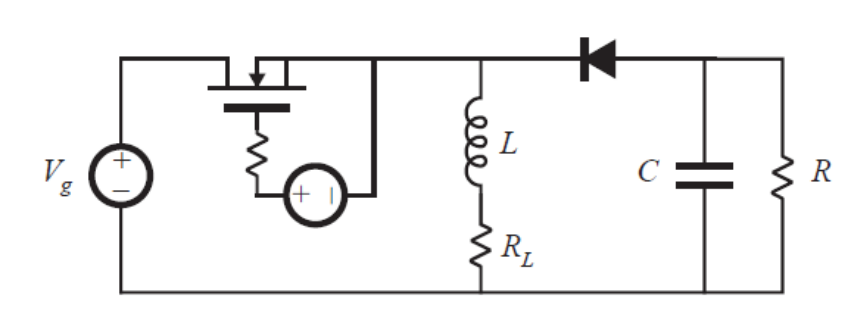
\includegraphics[width=10cm]{f3}
\end{center}
\end{figure}

We can begin by finding the average currents and voltages:
\[
  V_L = V_g - i_LR_L
\]
\[
  V_L = V - i_LR_L
\]
\[
  i_C = \frac{-V}{R}
\]
\[
  i_C = -i_L - \frac{V}{R}
\]
These make (including the equation for $i_g$):
\[
  0 = V_gD + VD'-I_LR_L
\]
\[
  0 = \frac{-V}{R} - I_LD'
\]
\[
  0 = DI_L+\frac{I_Lt_r}{T_S} + \frac{Q_r}{T_s}
\]

Our equivalent circuit will look like this:
\begin{center}
  \begin{circuitikz}[american]
    \draw
    (0,0) to[V=$V_g$] (0,3)
      to[short] (8,3)
    (0,0) to[short] (8,0)
      to[I=$I_LD'$] (8,3)
    (2,3) to[I=$\frac{I_Lt_r}{T_s}$] (2,0)
    (4,3) to[I=$\frac{Q_r}{T_s}$] (4,0)
    (10,3) to[V=$DV_g$] (10,0)
      to[short] (13,0)
      to[R=$R$] (13,3)
      to[R=$\frac{R_LD'^2}{D}$] (10,3)
    ;\end{circuitikz}
\end{center}
With a transformer:
\begin{center}
  \begin{circuitikz}[american]
    \draw
    (9,3) node[transformer](T) {} node[above] {${D'}^2 : 1$}
    (0,0) to[V=$V_g$] (0,3)
      to[short] (T.A1)
    (0,0) to[short] (6,0)
      to [short] (6, 0.9)
      to [short] (T.A2)

    (2,3) to[I=$\frac{I_Lt_r}{T_s}$] (2,0)
    (4,3) to[I=$\frac{Q_r}{T_s}$] (4,0)
    (11,0) to[short] (13,0)
      to[R=$R$] (13,3)
      to[R=$\frac{R_LD'^2}{D}$] (T.B1)
    (11,0) to[short] (11,0)
      to[short] (11,0.9)
      to[short] (T.B2)
    ;\end{circuitikz}
\end{center}



\end{document}
